% Copyright (c) 2014,2016,2018 Casper Ti. Vector
% Public domain.

\chapter{实验结果及分析}
%\pkuthssffaq % 中文测试文字。
\section{实验配置}
这一章测试了我们实现的 exFAT 文件系统的性能,并与 Linux 中的对应实现进行了比较。
由于目前 Asterinas 系统还处于开发阶段,还不能实机运行,只能使用 Qemu 进行测试。
故为了确保比较的公平,Linux 的实验结果也是通过 Qemu 取得。
另外,Linux 内核出于某些原因没有预设支持读写 exFAT 文件系统的驱动程序,下面的实验结果是通过 FUSE 套件取得,
可能对性能有一定影响,所以实验结果仅供参考。
我们进行的测试主要目的是测试文件 IO 性能,如果没有特殊说明,测试的默认情景是文件已经存在并且初始化完成,
页缓存在测试开始时为空,在这种情况下通过 FIO 触发文件读写并得到测试结果。
表\ref{tab:exp_setup}总结了本节实验的一些通用配置。

\begin{table}[h]
    \centering
    \begin{tabularx}{\textwidth}{|Y|Y|}
    \hline
    项目 & 描述 \\
    \hline
    存储设备大小 & 4G \\
    \hline
    系统内存大小 & 4G \\
    \hline
    测试文件大小 & 1G \\
    \hline
    单次请求大小 & 4K \\
    \hline
    FIO 测试读写引擎 & sync \\
    \hline
    Linux exFAT套件版本 & FUSE exfat 1.3.0+git20220115 \\
    \hline
    \end{tabularx}
    \caption{实验配置}
    \label{tab:exp_setup}
\end{table}

\section{exFAT文件系统性能测试}\label{sec:exp_file_io}

\begin{figure}[thbp!]
    \centering
    \begin{minipage}[t]{0.49\linewidth}
        \centering
        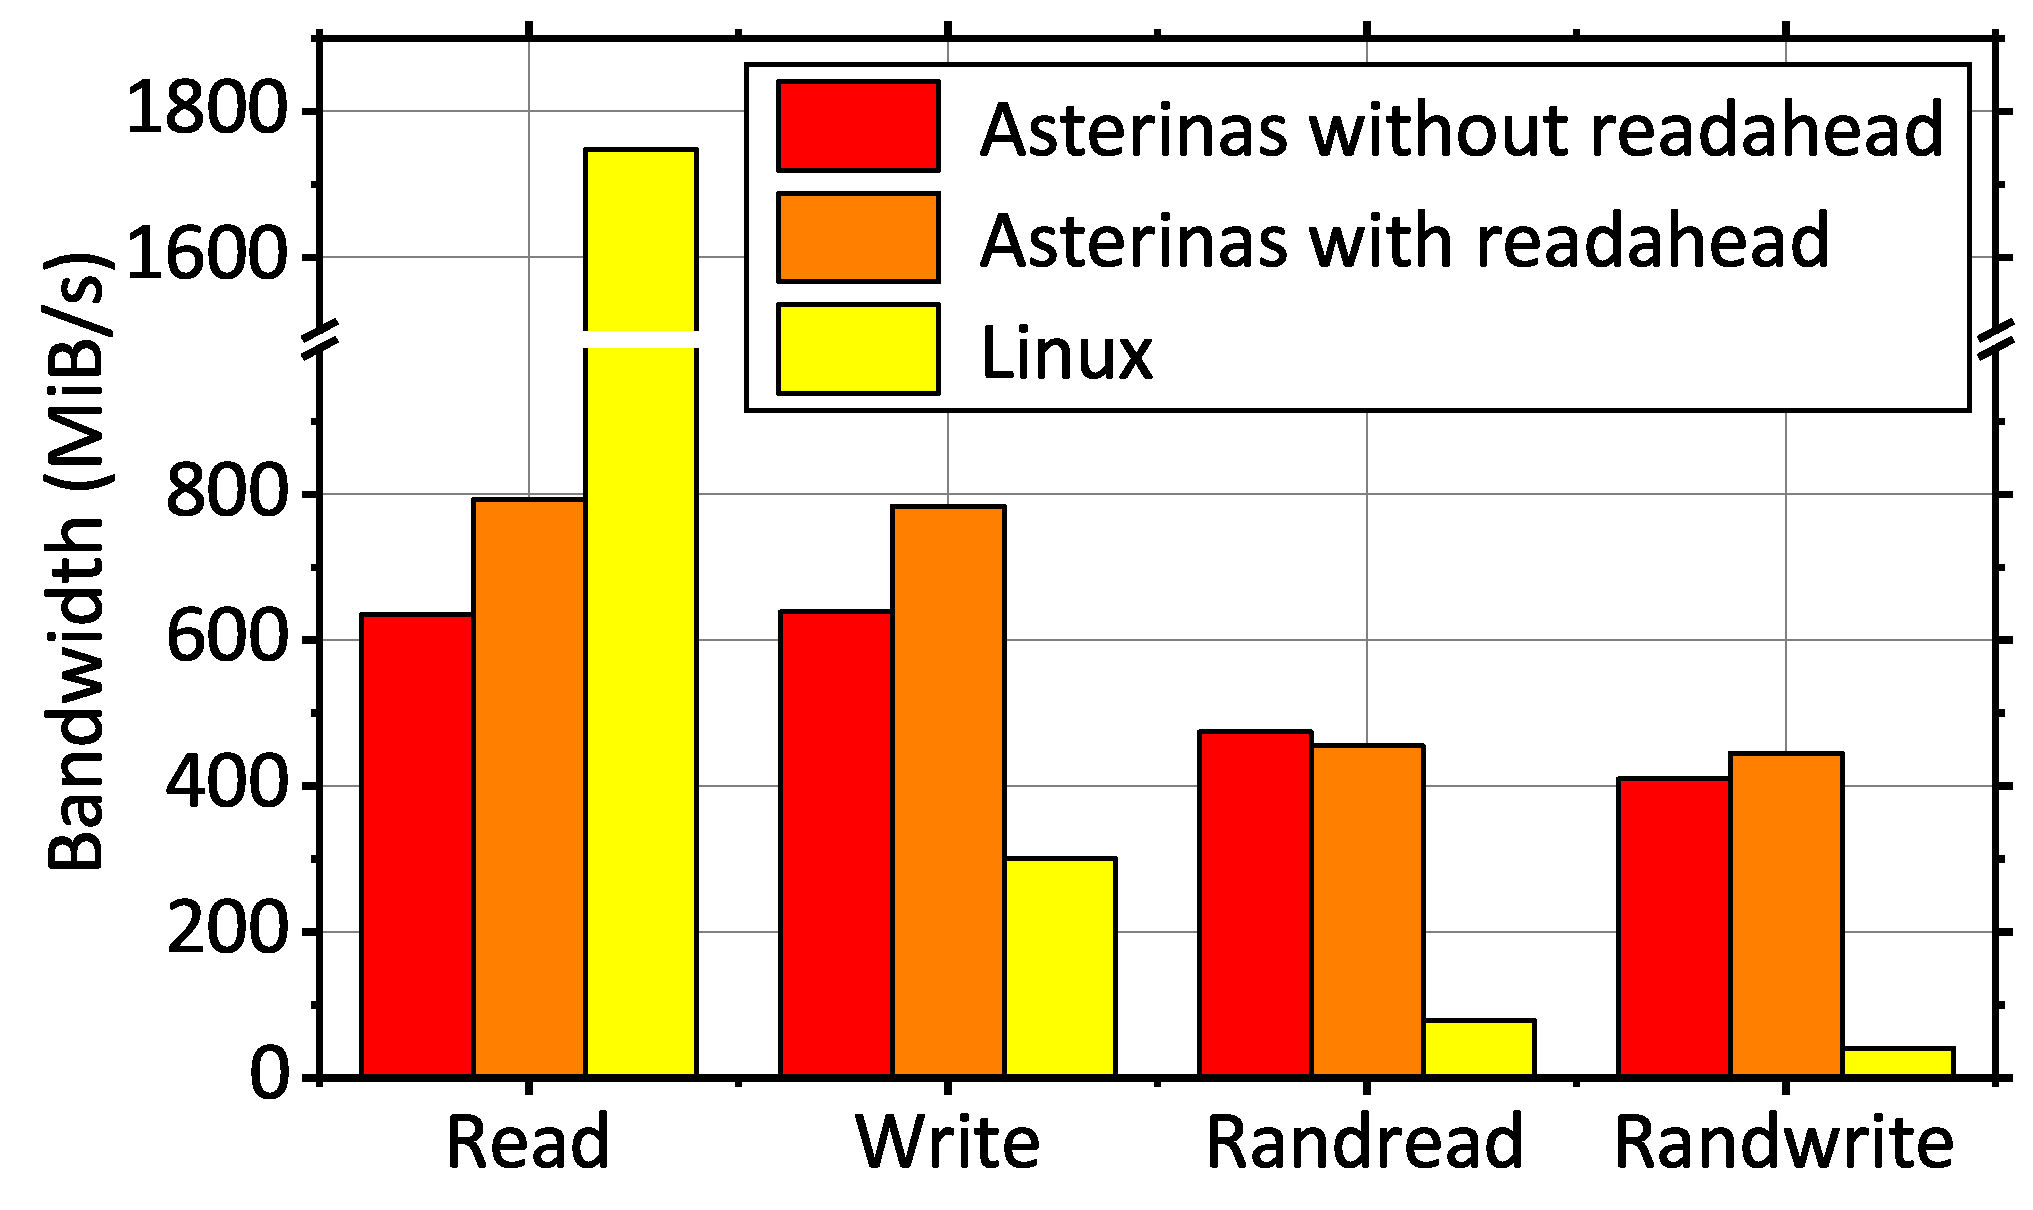
\includegraphics[width=0.9\linewidth]{cached_io.eps}
        \caption{使用页缓存的测试结果}
        \label{fig:cached_io}
    \end{minipage}
    \begin{minipage}[t]{0.49\linewidth}
        \centering
        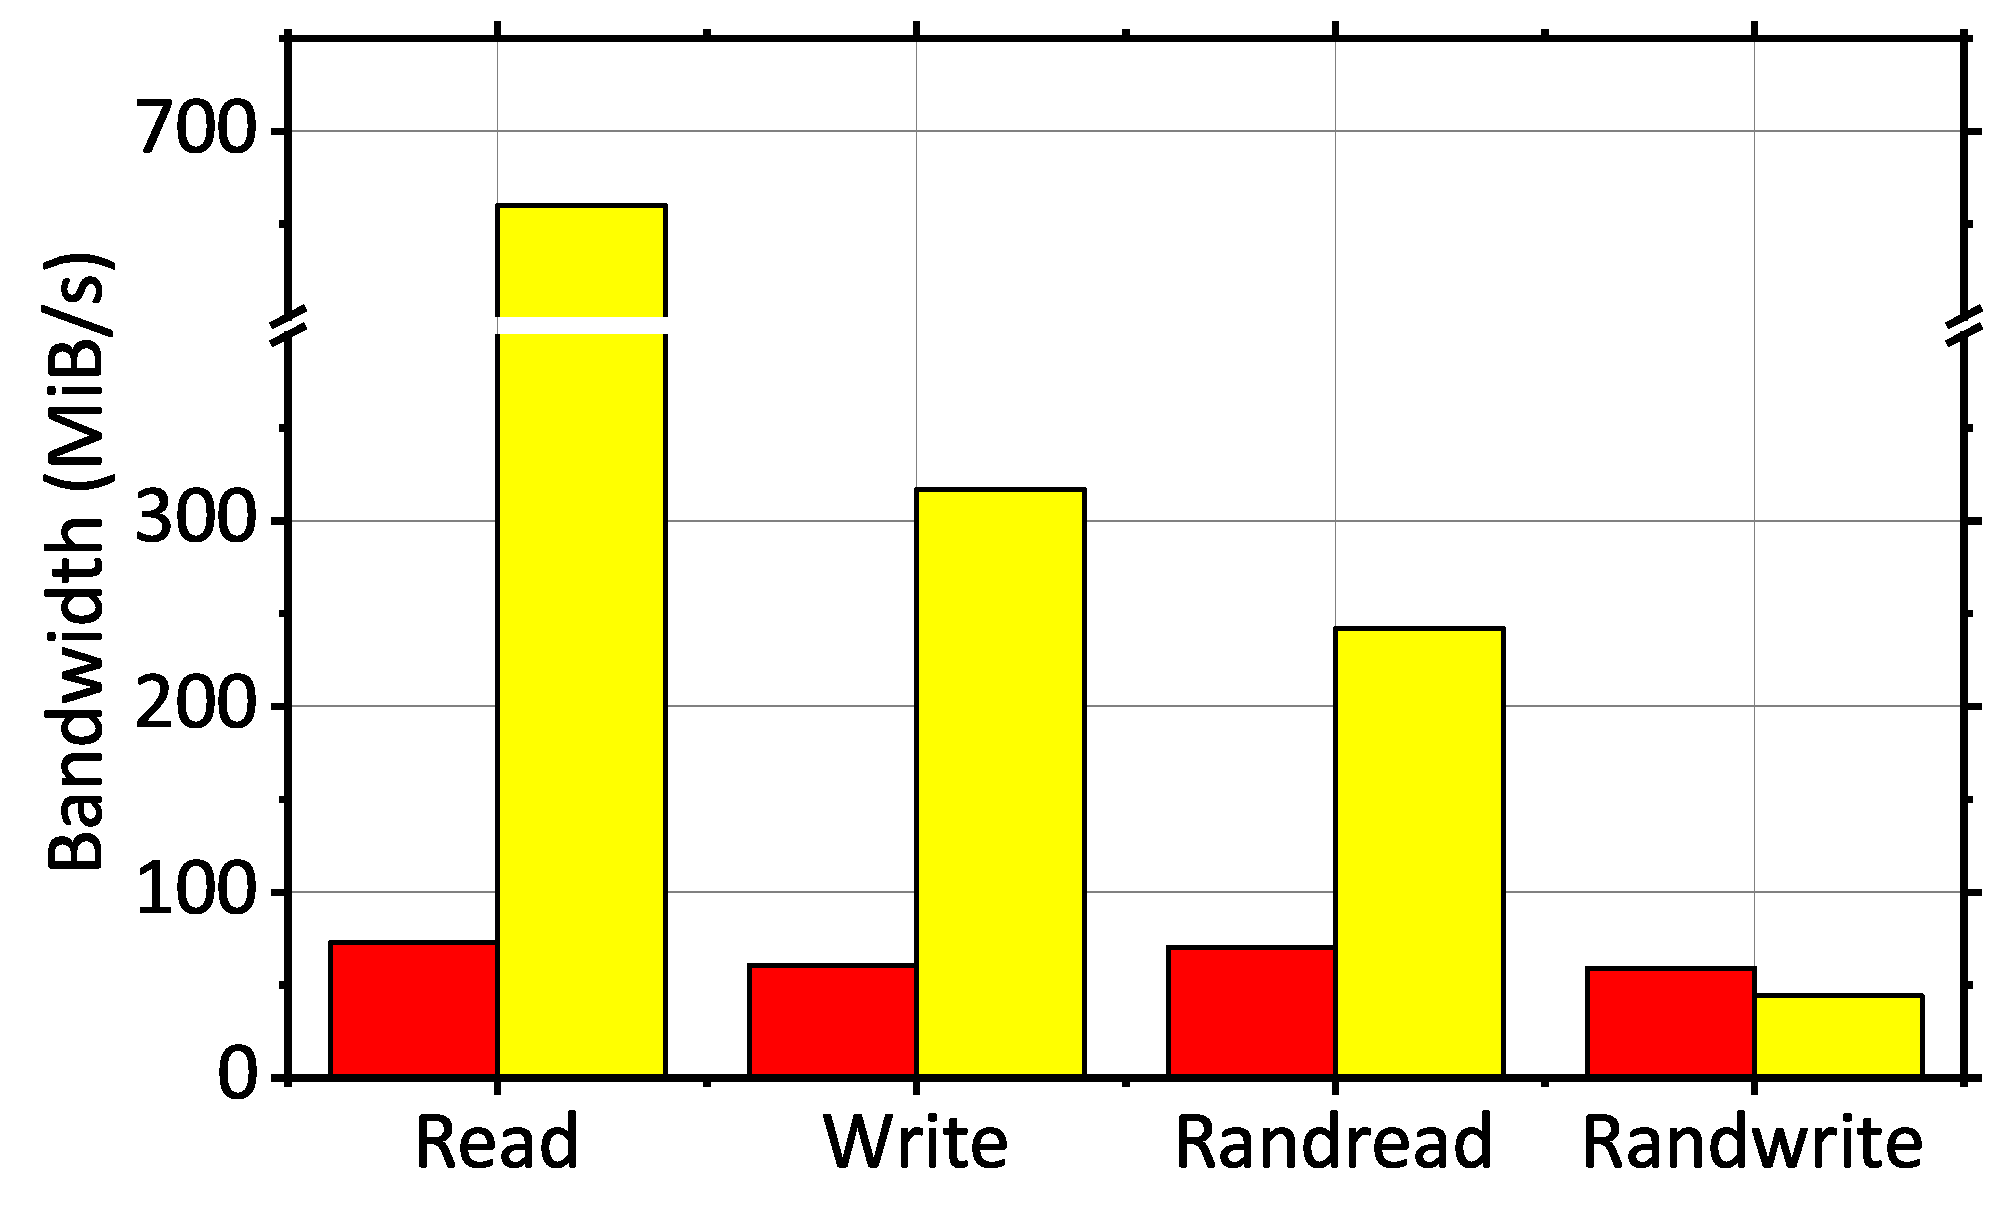
\includegraphics[width=0.9\linewidth]{uncached_io.eps}
        \caption{不使用页缓存的测试结果}
        \label{fig:uncached_io}
    \end{minipage}
 \end{figure}

我们比较了在不同读写模式下,初始页缓存为空的状态下,以单次请求大小为粒度,对测试文件进行连续 60s IO 操作的平均带宽。
图\ref{fig:cached_io}展示了使用页缓存情况下的 IO 带宽,分别比较了使用数据预取的 Asterinas 系统、不使用数据预取的 Asterinas 系统以及 Linux 系统
在顺序读、顺序写、随机读、随机写模式下的 IO 带宽。
图\ref{fig:uncached_io}则展示了不使用页缓存的情况下的 IO 带宽, 仍然是比较了Asterinas 系统(这时是否使用数据预取没有区别)
和 Linux 系统在四种 IO 模式下的带宽。

从图\ref{fig:cached_io}中可以看出,在使用页缓存的情况下,页缓存预取机制的引入提高了顺序访问模式下的 IO 带宽,
而随机访问模式的 IO 带宽没有受到明显影响,整体的 IO 表现符合预期。
此外,通过和 Linux 的对比可以看出,我们的实现在顺序读模式下明显慢于 Linux,但其余 IO 模式都优于 Linux。
考虑到 Linux 的实验结果是通过 FUSE 套件取得,会对性能有一定影响,故这个比较仅供参考。
本节的测试均是连续做 IO 60s 得到的平均性能,从下一节的测试中也能看出,在引入数据预取之后,我们测得的平均性能已经接近峰值性能。
这说明测试文件随着测试的进行会被完全放入页缓存,在这种情况下,因为文件已经被完整缓存,文件系统不会向块设备层发送 IO 新的请求。
但测出的顺序读性能仍然低于 Linux 中的实现,所以页缓存仍有改进的空间。
在不使用缓存的情况下,所有的 IO 均直接与底层块设备进行交互,自然会慢于使用页缓存的结果。
图\ref{fig:uncached_io}中的测试结果表明,Asterinas 系统直接读写块设备的速度普遍慢于 Linux 系统,
这其中可能的原因是测试时的 Asterinas 系统还处于研发初期,其中的块设备层只能支持同步 IO,
而 Linux 系统的块设备层存在异步 IO 以及一些优化策略。

\section{数据预取性能测试}

为了进一步观察我们为页缓存实现数据预取所带来的性能提升,我们又测试了在两种不同的页缓存配置下,使用各种不同的 IO 模式,
对同一文件进行的连续十次相同 IO 的性能变化。
每次 IO 定义为使用相应的读写模式,以单次请求大小为粒度,总计请求和测试文件大小相同的数据。
在第一次 IO 开始前,页缓存是空的,此后的每一次测试都是紧接着前一次测试进行,不清空页缓存。

\begin{figure}[h]
    \centering
    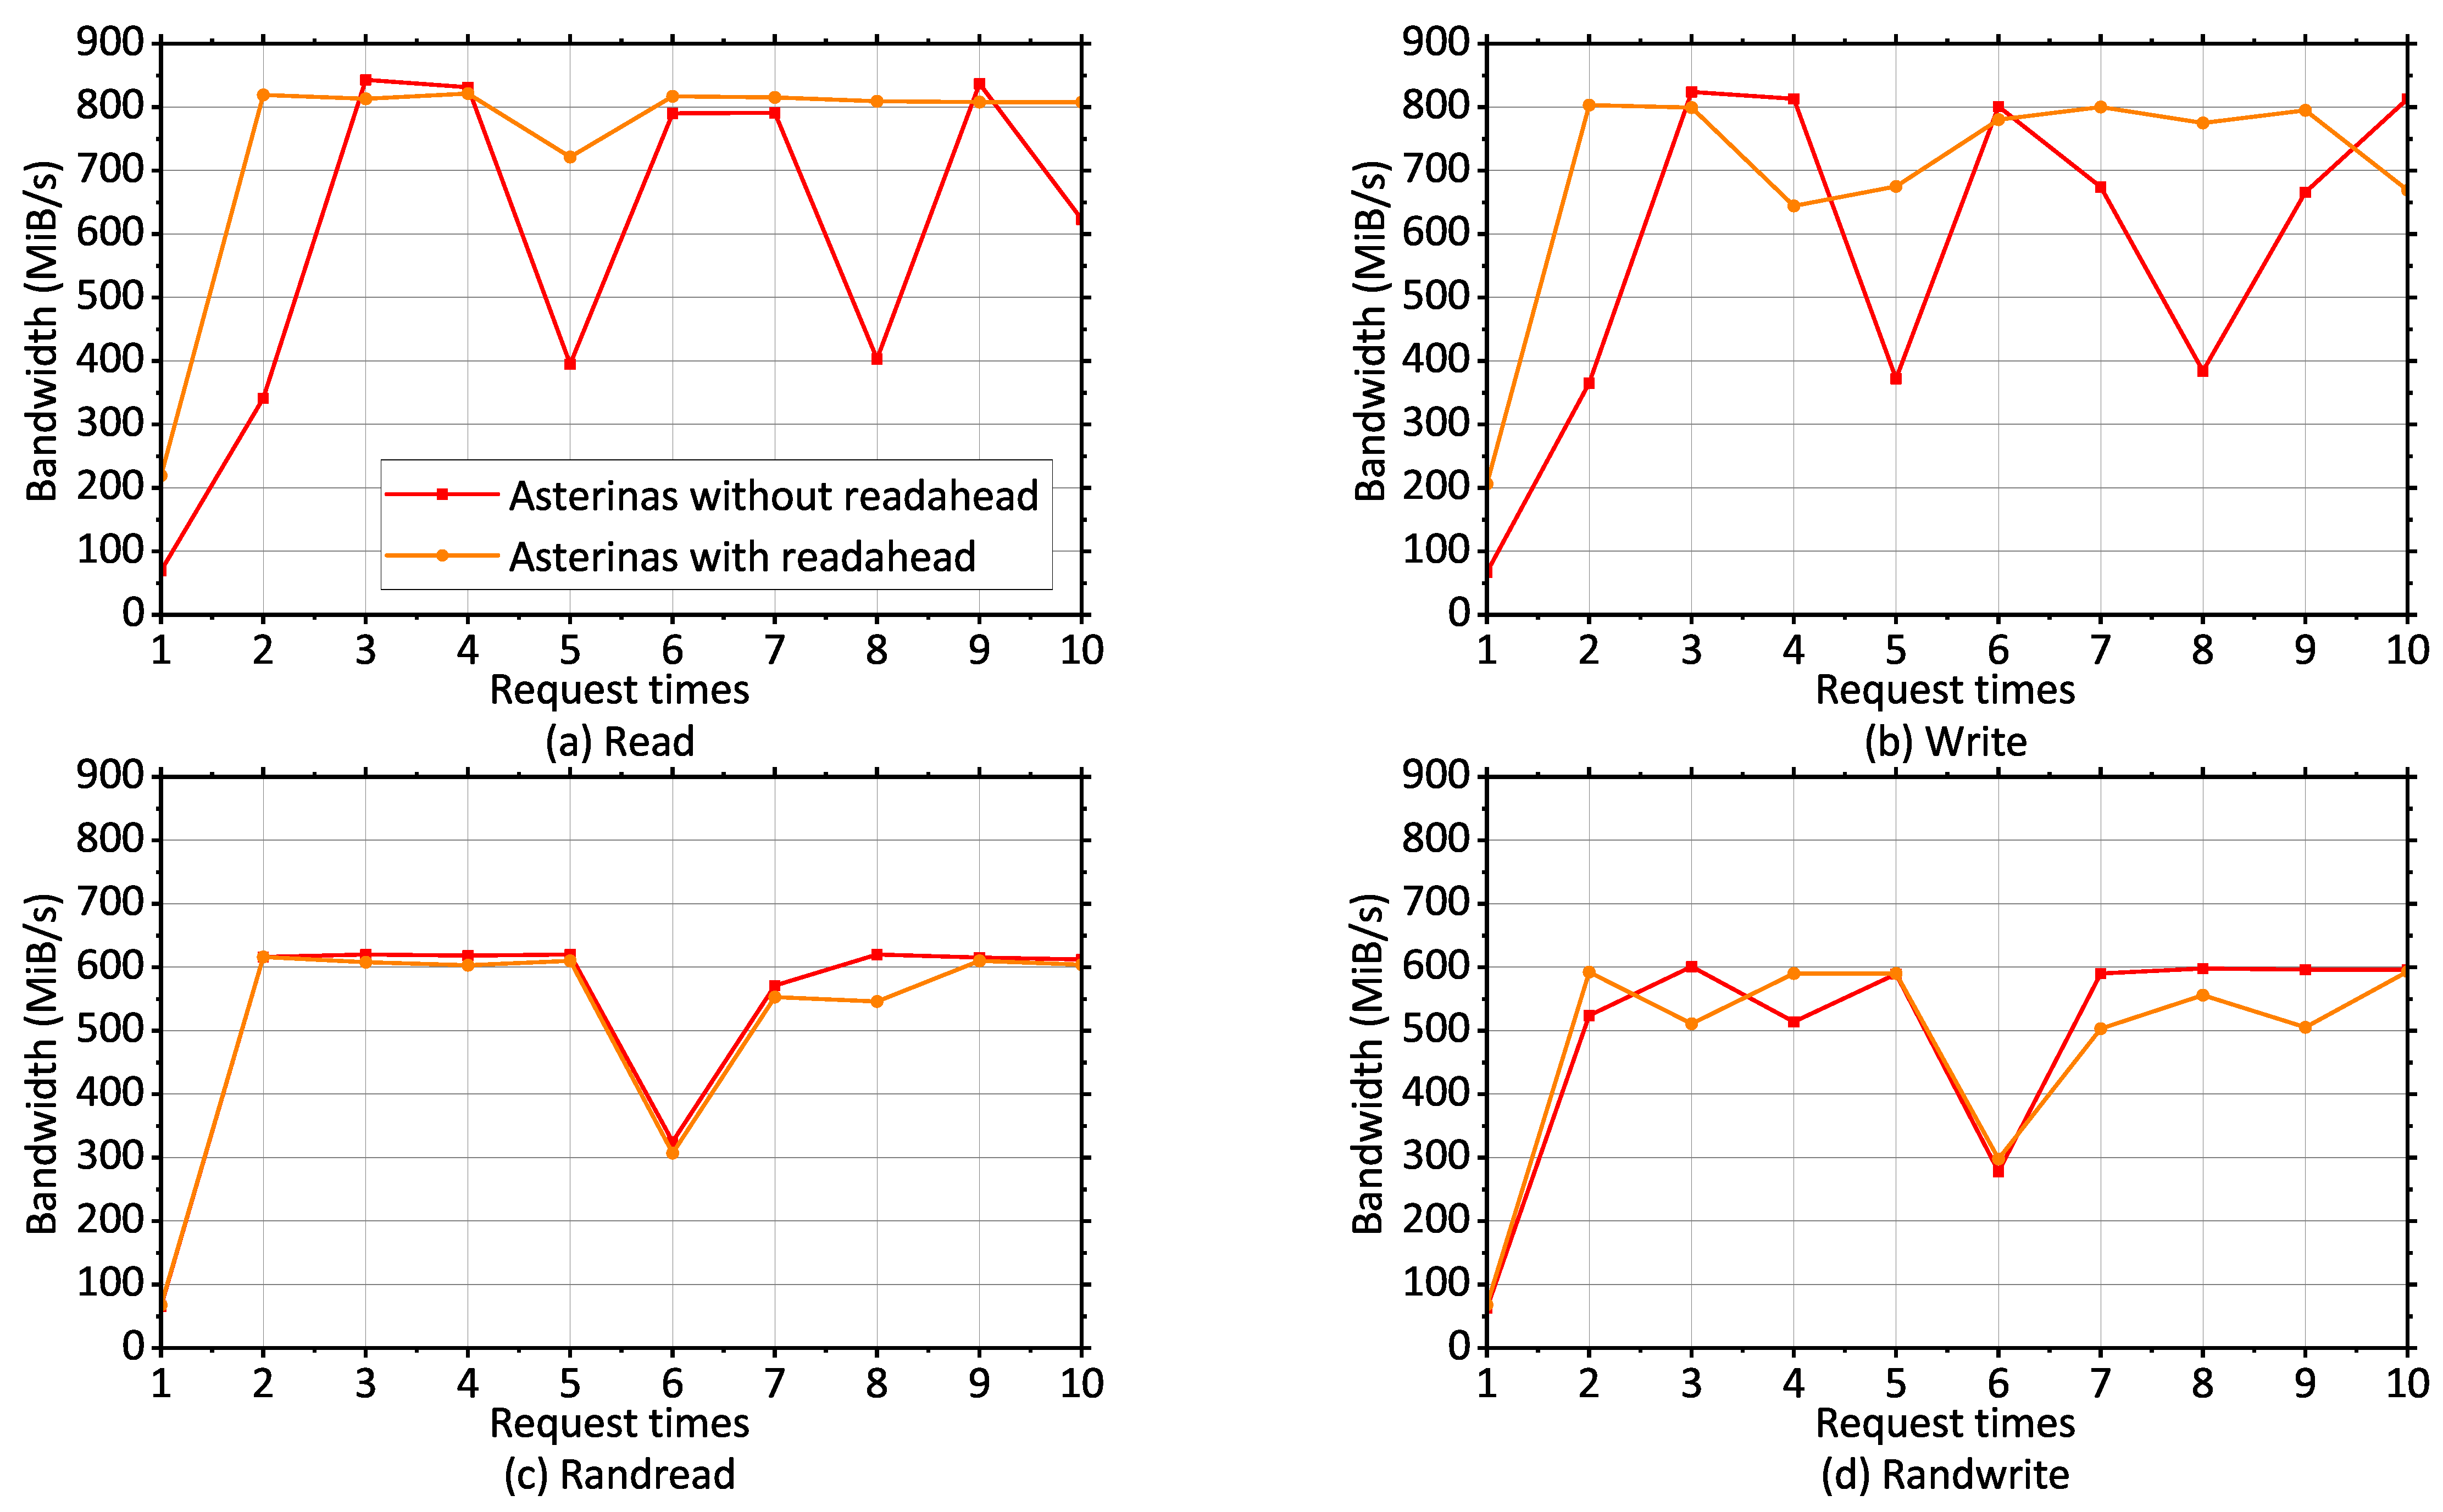
\includegraphics[width=1.0\textwidth]{cmp_combined.eps}
    \caption{使用数据预取与否对性能的影响}
    \label{fig:cmp_ra}
\end{figure}

图\ref{fig:cmp_ra}中展示了我们的测试结果,每张图对应一种 IO 模式,图中的两根曲线分别代表使用数据预取和不使用数据预取的 Asterinas 系统。
从图中可以看出,我们的数据预取的引入主要提升的是顺序 IO 模式的性能表现,对于随机 IO 模式,是否使用数据预取对性能影响不大。
对于顺序 IO 模式,使用数据预取能更快的达到性能峰值,此外,还可以减少性能的波动,使性能维持在峰值附近。
这个结果与\ref{sec:exp_file_io}节的实验结果相符,正是因为 IO 性能能更快的达到峰值,才使得增加数据预取后的总的 IO 性能得到提升。
但从图中还可以看出,我们的数据预取仍有提升的空间,在最理想的情况下顺序 IO 的性能可以在首次调用时便达到峰值,
在这种情况下,上层应用可以完全感知不到块设备层的存在,对于上层应用来说,文件仿佛始终位于内存之中。
这可能是因为测试时 Asterinas 系统的块设备层仍是同步的实现,对此继续改进的方向可能是为块设备层提供异步 IO 支持。
% vim:ts=4:sw=4
